\documentclass{llncs}

\usepackage{graphicx}                                        % for pdf, jpeg, png and tif graphics
\usepackage{amsmath}                                         % for align
\usepackage{amssymb}                                         % for >= and <= signs
\usepackage{xfrac}                                           % for nice x/y fractions (sfrac)
\usepackage{tikz}
\usepackage{amsbsy}                     % for boldsymbol
\usepackage{upgreek}

\mathchardef\mhyp="2D    % define math mode hyphen

\allowdisplaybreaks[4]

\title{Deep feedback learning}

\author{Bernd Porr \and Paul Miller}

\institute{Glasgow Neuro, bernd,paul@glasgowneuro.tech}

\begin{document}

\maketitle

\begin{abstract}
\end{abstract}

\section{Introduction}

\begin{figure}[h!]
  \centering
  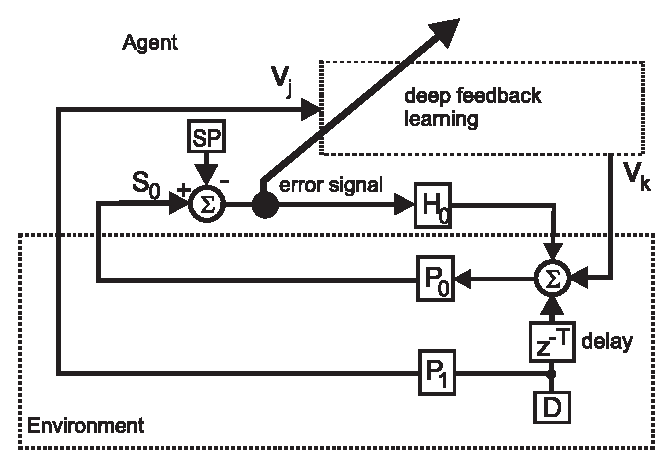
\includegraphics[width=0.75\columnwidth]{closed_loop}
  \caption{A closed loop system with a setpoint $SP$, transfer function $H$ and the
    environment $P_0$ which needs to work against unpredictable disturbances $D$.
    The error signal generated tunes a deep neuronal network which has inputs
    $v_j$ which predict the disturbances. The network tries to pre-empt these
    disturbances and generate an appropriate action $v_k$.
    \label{closed_loop}}
\end{figure}

\section{Closed loop learning}

Deep feedback learning operates in a closed loop scenario. Before we can describe
the actual deep feedback algorithm we need to put the algoritm into a closed loop
system. Fig.~\ref{closed_loop} shows the whole closed loop system with the deep
feedback learning as a black box for now. The main idea is that we have a fixed
closed loop which is able to fend off disturbances. For example this can be
an unexpected bend on a road or the sudden appearance of an enemy. The loop then
takes appropriate action to solve this disturbance, e.g. steering the car along
the road or shoots the enemy. In formal terms we have a setpoint $SP$ which
compares the input of organism to an input. If that input deviates from the
setpoint an action is generated with the transfer function $H_0$. This action
then eliminates the disturbance $D$ and arrives via the environmental
transfer function $P_0$ at the input again, thus, the loop is closed. However,
we are not so much interested in the particular design of the the closed loop
but that it generates an \textsl{error signal}. This error signal is non-zero
if a disturbance has happend. This error signal can now be used to tune our
deep feedback learning network.

The deep feedback learning network receives additional inputs which are able
to predict the disturbance and thus can prevent the trigger of the feedback
loop. These additional inputs are provided via the transfer function $P_1$
and represent the disturbance in a filtered form. For example a video camera
can provide images of the road ahead or that of the enemy. Deep feedback
learning has the task to take the error signal and tune its network
to generate an action which helps to minimise the error. In the next section
we are going to describe the deep feedback learning now how this can
compute the appropriate output. Note that deep feedback learning receives
its feedback via the environment so that it only learns if it has been
successful after its actions have travelled through the environment. Thus learning
evaluates if certain inputs to its network can be used to generate
appropriate actions and these are then slowly transformed into actions.
For that reason the error signal is propagated in a \textsl{forward} fashion
throught the network which will be presented next.

\begin{figure}[h!]
  \centering
  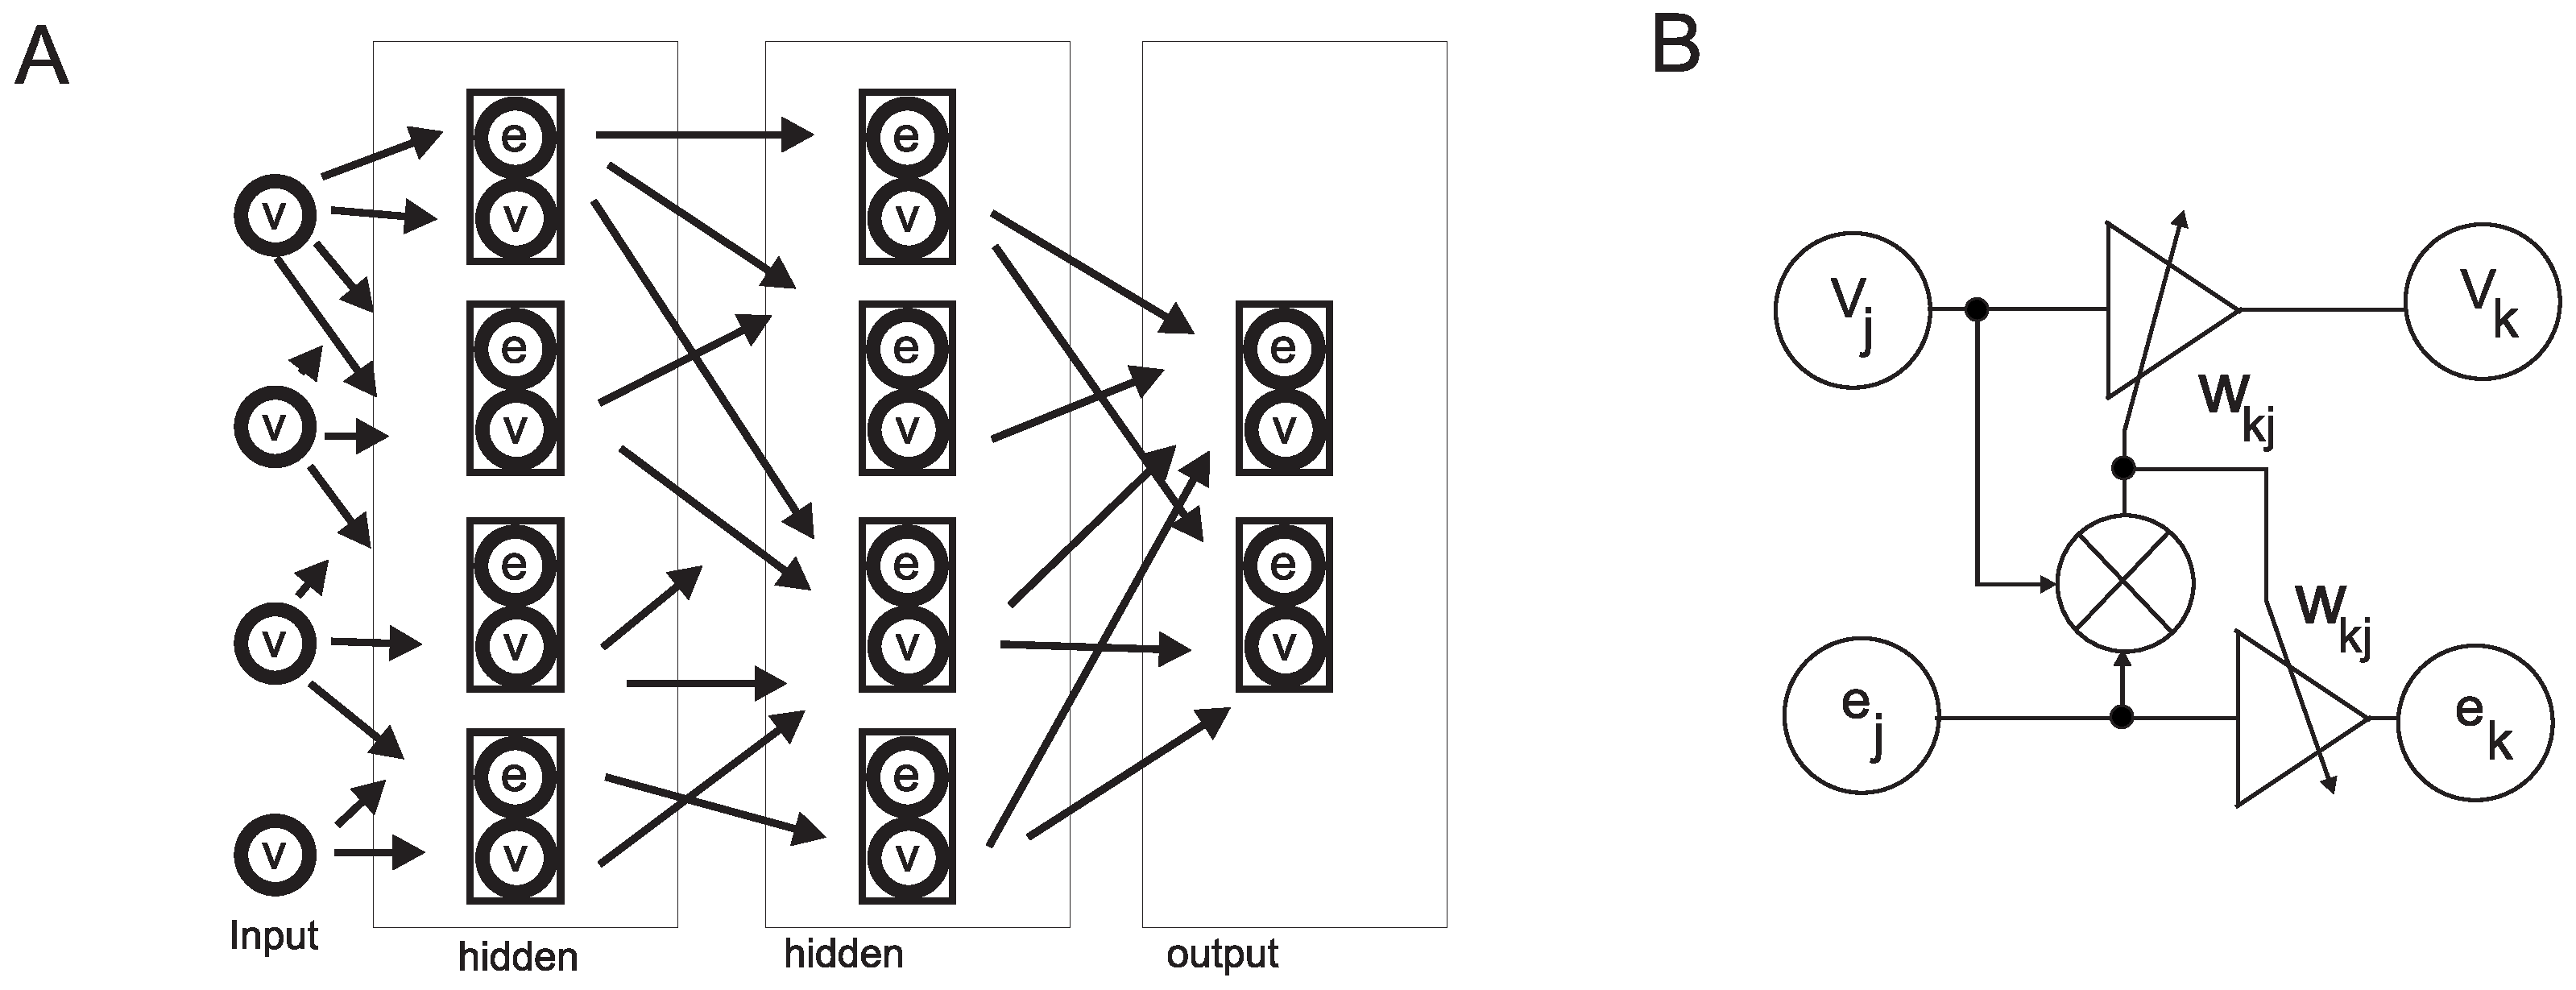
\includegraphics[width=\columnwidth]{netw_together}
  \caption{A) Overview of the network. Except for the input layer
    every neuron is a composite neuron with an activation $v$ and
    and an error term $e$. These are propagated through the network
    in a weighted fashion in parallel.
B) Computation in a single cell composite cell in the network.
    The presynaptic activities $v_k$ and error signals $e_k$ are used
    to perform correlation based learning and change the weight $w_{kj}$
    which weights both the activity and the error towards the next
    layer.\label{netw_together}}
\end{figure}


\section{Deep feedback learning}
We define a network with an input layer, hidden units and an output
layer which can all have different number of neurons (see
Fig~\ref{netw_together}A). However, in contrast to traditional
networks every layer (except for the input layer) consists of two
summation nodes: the actual activity and an error signal. These
are processed in two parallel streams.

Let us first focus on the calculation of the network activity and then
we deal with the error processing. We define a multi layered network
where every neuron is a standard computational unit which calculates
the weighted sums of its inputs and then sent through an activation
function:
\begin{equation}
  v_k = \Theta\left( \sum_i w_{jk} v_{j} \right) \label{act_sum}
\end{equation}
where the activity feeds from neurons in layer $v_j$ to neurons in layer $v_k$
and so forth. The activities are weighted by the weights $w_{jk}$
in a standard fashion.

The weight change is then calculated in a semi Hebbian fashion:
\begin{equation}
  w_{jk} = w_{jk} + \gamma v_j * e_k
\end{equation}
where $v_j$ is the presynaptic activity and $e_k$ is the error signal
attached to the postsynaptic neuron so that the correlation is
calculated between the input signals and the error signals. This is similar
to Hebbian learning but here the presynaptic term is the activity
and postsynaptic one is the error signal.

The error signal needs to be described in more detail how this
is propagated through the network. As described above the error
signal emerges from the feedback loop which is injected into the
network at its first hidden layer as the ``postsynaptic'' activity.
Since the 1st hidden layer directly receives its error signal this
can be computed instantly.

For the deeper layers the error signal is computed as a weighted
sum of the error signals from the previous layer:
\begin{equation}
  e_k = \frac{\left( \sum_j w_{jk} e_{j} \right) \Theta^\prime (v_k) }{\sqrt{\sum_j w_{jk}}}
\end{equation}
where the $\Theta^\prime (v_k)$ is the derivative of the activation
function $\Theta(v_k)$.

The computations performed in every layer are shown in
Fig~\ref{netw_together}B where we see that the activity $v_j$ is
weighted by the weight $w_{jk}$ and then summed up in the next
layer. The same happens for the error signal $v_j$ which is also
weighted by $w_{jk}$. Remember that for the 1st hidden layer this
error signal is just the injected error signal from the feedback loop
and is not the weighted sum.

Learning is then performed in three steps: first the activity is propagated through
the network, then the error signal is propagated via the same mechanism and then the
weights are adjusted. Thus, both the error
signal and the activity is propagated in a forward fashion through the network.
Learning itself is the ``Hebbian'' but by correlating the actual activation
and the error signal. 

\begin{figure}[h!]
  \centering
  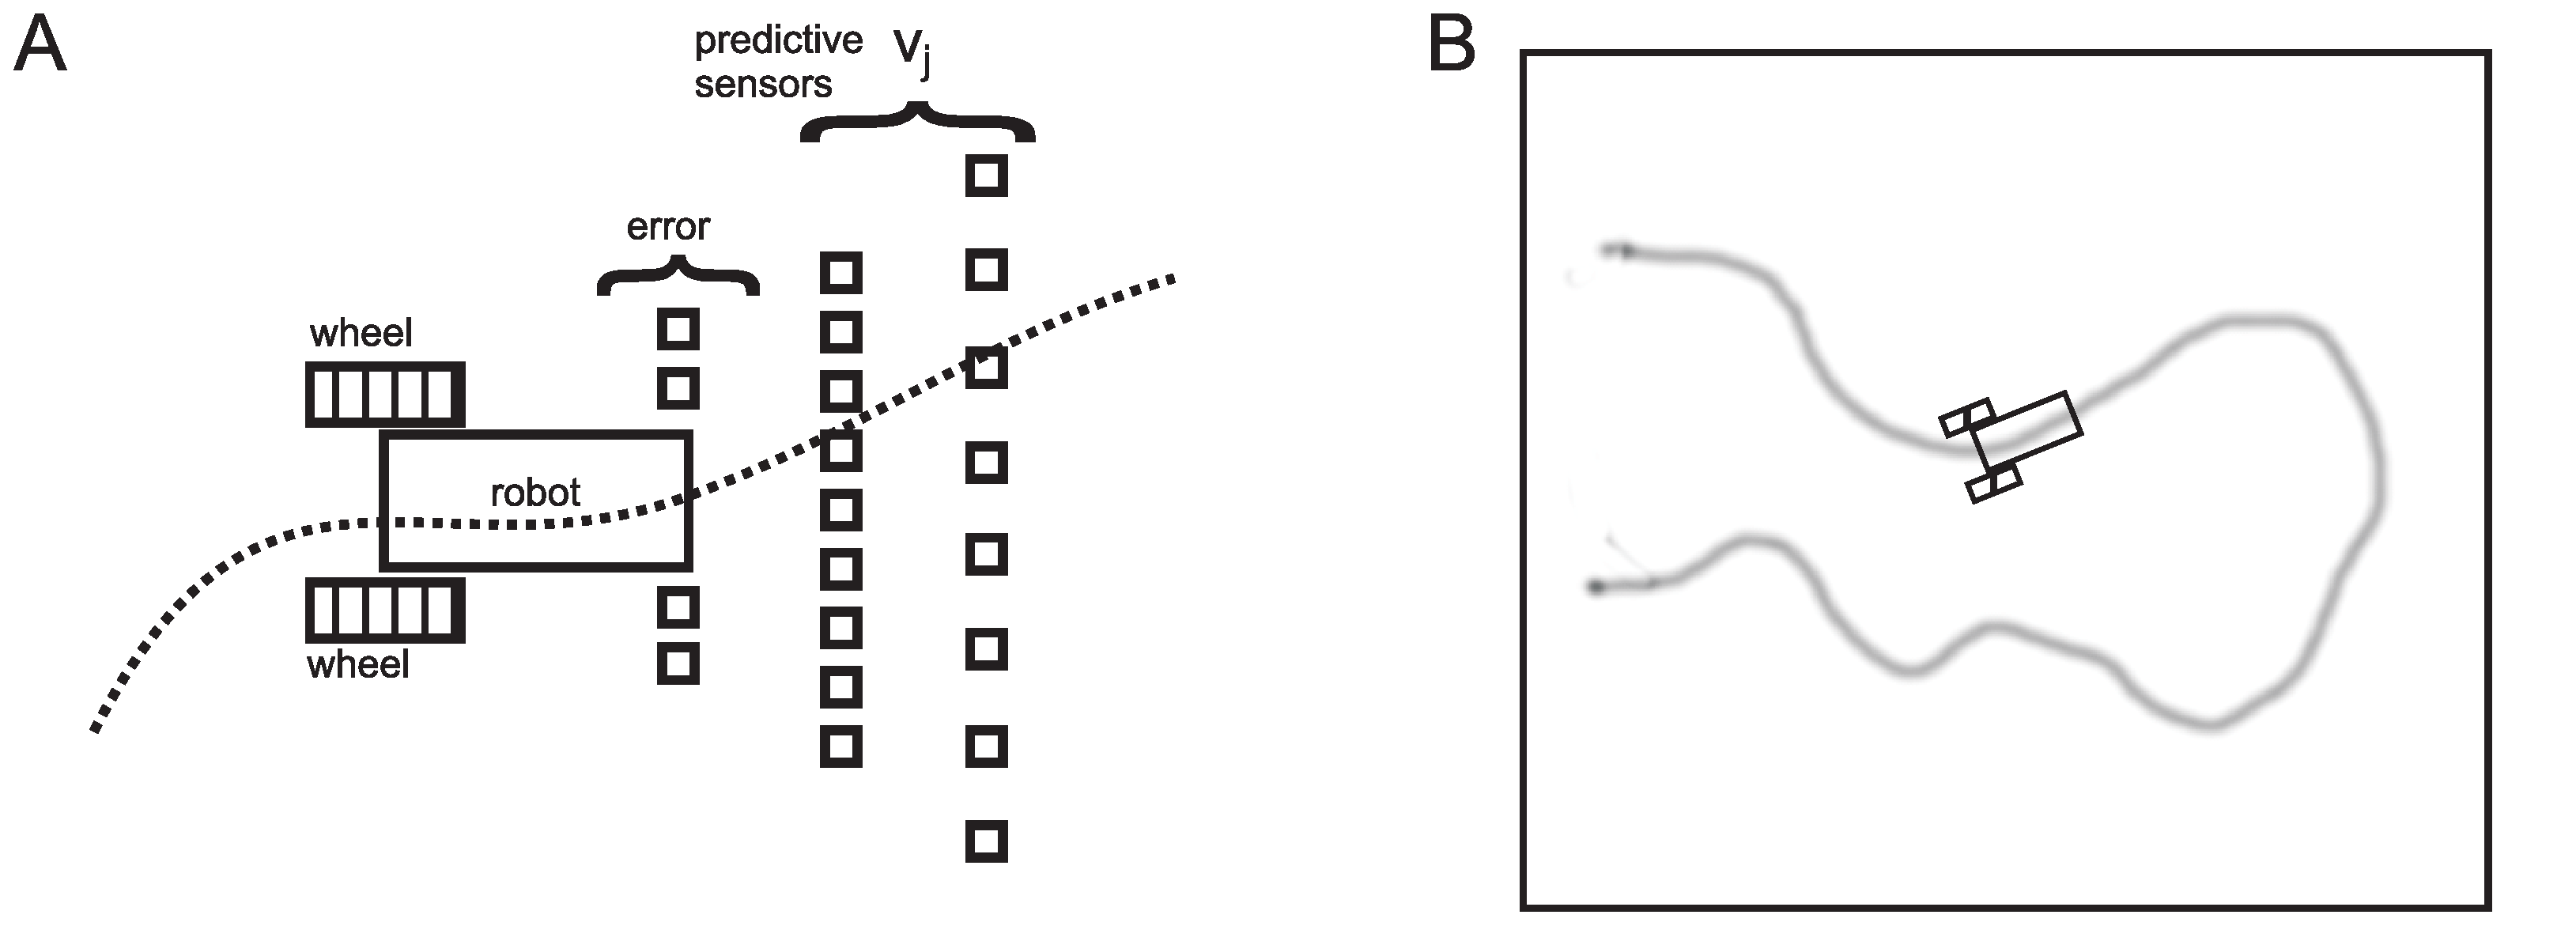
\includegraphics[width=\columnwidth]{linefollower_robot_playground}
  \caption{A) Robot setup. The robot is simulated with a updated
    version of enki for QT5 (https://github.com/berndporr/enki)
    where the line follower is using just the ground sensors of the
    robot to create the error signal and the predictive signals ($v_j$)
    for DFL. The robot has two wheels which speed is controlled
    by the feedback control and DFL.
    B) The line following scenario used for the simulations. The robot
    attempts to drive along the line and is reversed at the end of the
    line and the drives back. If it hits the boundaries of the playground
    it is also turned around.
    \label{linefollower_robot_playground}}
\end{figure}




\section{Line follower}
In order to demonstrate DFL we need a simple closed loop scenario which can be
improved with the help of our adaptive neuronal network. 
Fig.~\ref{linefollower_robot_playground} shows a simple line following robot which has the task to
follow the line as depicted in
Fig.~\ref{linefollower_robot_playground}B wheret the robot at the end the robot is reversed
and then drives it back in the other direction and so forth. The 4 ground sensors
in Fig.~\ref{linefollower_robot_playground}A right to both sides of the robot create
an error signal:
\begin{equation}
\mathrm{error} = (g_{l_1}+2 g_{l_2})-(g_{r_1}+2 g_{r_2})
\end{equation}
which then directly create a steering reaction to keep the robot on track by
controlling the speed of the wheels. Without taking into account the contribution
of our deep feedback learning output this yields: $\mathrm{leftSpeed} = s_0 + g error$ for the
left wheel and $\mathrm{rightSpeed} = s_0 - g error$ for the right wheel
where $s_0$ is the baseline speed of the robot and $g$ the feedback gain. We now
need to add the deep feedback learning circuit to it.

We now need to add our deep feedback learning circuit which uses the
predictive ground sensors where their outputs all feed into $v_j$ of
the input layer (see Eq.~\ref{act_sum}). We have two rows of sensors. One which
is right in front of the robot and another one which looks further ahead.

The output layer of our deep feedback learner with its activations
$v_k$ has 6 neurons ($k=0 \ldots 5$) which can be seen as soft
decision making units where 3 of them determine the change of the speed of
the wheel on the right and 3 of them the speed of the wheel on the
left which leads to the final formulas for the motor outputs:
\begin{eqnarray}
\mathrm{leftSpeed} &= s_0 + g\, \mathrm{error} + &\left( 50 v_0 + 10 v_1 + 2 v_2 \right) \\
\mathrm{rightSpeed} &= s_0 - g\, \mathrm{error} + &\left( 50 v_3 + 10 v_4 + 2 v_5 \right)
\end{eqnarray}
where $v_0, \ldots, v_5$ are the 6 outputs from the deep feedback learning network.
Note that neither the inputs nor the outputs are organised in a topographically
organised way. The network needs to find out with the help of the error signals
which sensor inputs $v_k$ will lead eventually to appropriate steering actions $v_j$.


\subsection{Results}


\section{Shooter game}


\subsection{Results}


\section{Discussion}

\bibliographystyle{splncs03}

\bibliography{sab_submission,isab,ours}

\end{document}



\begin{figure}[h!]
  \centering
  \includegraphics[width=\columnwidth]{arena_cct.pdf}
  \caption{A. Overview of the simulation environment. The arena has two markers, labelled R and B (red and blue), within   \label{fig:cct}
    }
\end{figure}

